\pdfminorversion=4
%\documentclass[prodmode,acmtrets]{acmsmall}
\documentclass[acmtrets]{acmsmall}
\usepackage[binary-units]{siunitx}
\usepackage{algorithm}
\usepackage{algorithmic}
\usepackage[algo2e]{algorithm2e}
\renewcommand{\algorithmcfname}{ALGORITHM}
\SetAlFnt{\small}
\SetAlCapFnt{\small}
\SetAlCapNameFnt{\small}
\SetAlCapHSkip{0pt}
\IncMargin{-\parindent}

% Metadata Information
\acmVolume{0}
\acmNumber{0}
\acmArticle{1}
\acmYear{2014}
\acmMonth{0}

\usepackage{amsmath}
\usepackage[flushleft]{threeparttable}
\usepackage[shortlabels]{enumitem}
\usepackage{graphicx}
\usepackage{multirow}
\usepackage[caption=false,font=footnotesize]{subfig}
\usepackage{dblfloatfix}
\usepackage{xspace}
\usepackage{url}
\usepackage[square, comma, sort&compress, numbers]{natbib}

% \usepackage{draftwatermark}%
% \SetWatermarkFontSize{20cm}%
% \SetWatermarkScale{2}%
% \SetWatermarkText{DRAFT Do not distribute}%

\setlength{\parskip}{0pt}
\renewcommand{\topfraction}{1}
\renewcommand{\textfraction}{0.15}
\renewcommand{\dbltopfraction}{1}

\renewcommand\floatpagefraction{.9}
\renewcommand\topfraction{.9}
\renewcommand\bottomfraction{.9}
\renewcommand\dbltopfraction{.9}
\renewcommand\textfraction{.1}   
\setcounter{totalnumber}{4}
\setcounter{topnumber}{8}
\setcounter{bottomnumber}{4}
\setcounter{dbltopnumber}{4}

\newcommand{\eqnref}[1]{(\ref{#1})}
\newcommand{\figref}[1]{Figure~\ref{#1}}
\newcommand{\algref}[1]{Algorithm~\ref{#1}}
\newcommand{\secref}[1]{Section~\ref{#1}}
\newcommand{\tabref}[1]{Table~\ref{#1}}
\newcommand{\code}[1]{\texttt{#1}}

\newcommand{\tabincell}[2]{\begin{tabular}{@{}#1@{}}#2\end{tabular}}

\graphicspath{{./figures/}}

\begin{document}

\markboth{C.Liu et al.}{QuickDough: A Rapid FPGA Accel. Design Framework Using SCGRA Overlay}

\title{QuickDough: A Rapid FPGA Accelerator Design Framework Using Soft Coarse-Grained Reconfigurable Array Overlay}
\author{CHENG LIU
\affil{The University of Hong Kong}
COLIN YU LIN
\affil{The University of Hong Kong}
HAYDEN KWOK-HAY SO
\affil{The University of Hong Kong}
}

\begin{abstract}
    The QuickDough design framework is presented as a way to address productivity issues of developing
high-performance FPGA accelerators. QuickDough utilizes a soft coarse-grained reconfigurable array
(SCGRA) as an overlay on top of off-the-shelf FPGAs for rapid accelerator developments.
Instead of compiling high-level applications directly to HDL circuits, the compilation step is
reduced to a simpler operation scheduling task targeting the SCGRA overlay, significantly reducing
compilation time and increasing possible numbers of debug-cycle-per-day as a result.
The softness of the SCGRA allows highly customized application-specific design while the regular
structure of the SCGRA makes the customization much easier. When compared to the
execution on a general purposed processor, the accelerators generated using QuickDough achieves up
to 9X performance speedup.

\end{abstract}

\terms{Design, FPGA, Overlay, CGRA}
\keywords{Overlay, FPGA Accelerator, Soft Coarse 
Grain Reconfigurable Array, Design Productivity}

\acmformat{Cheng Liu, Colin Yu Lin, and Hayden Kwok-Hay So, 2014. 
QuickDough: A Rapid FPGA Accelerator Design Methodology Using Soft 
Coarse-Grained Reconfigurable Array Overlay.}

\begin{bottomstuff}
This work is supported in part by the Research Grant Concil of Hong
Kong, under the General Research Fund project 716510 and in part by
the Croucher Innovation Award of the Croucher Foundation.

Author's addresses: Cheng Liu, Colin Yu Lin, and Hayden Kwok-Hay So
Department of Electrical and Electronic Engineering, The University of
Hong Kong, Pokfulam Road, Hong Kong

\end{bottomstuff}

\maketitle

\section{Introduction}
Offloading compute intensive nested loops to FPGA accelerators has 
been demonstrated as an effective way of performance 
acceleration across various application domains\cite{Chung2010}. 
However, the design productivity of developing such accelerators 
remains relatively low and it has become a major obstacle that 
hinders the wide adoption of FPGAs as compute engines. Although the use of 
high level synthesis (HLS) tools which allow the application designers to 
focus on high level functionality instead of low-level implementation details alleviates 
this shortcoming \cite{cong2011high}, the lengthy low-level FPGA implementation process 
greatly limits the number of compile-debug-edit cycles per day and dramatically 
affects the overall design productivity. 

To approach the above design productivity problem, 
researchers have recently turned to the use of virtual FPGA overlay 
architectures \cite{Grant2011Malibu,ZUMA2012,mesh-FUs,
ferreira2011fpga, kissler2006dynamically,scgra}. When combined properly to 
high level compilation tools, the overlay architecture based design methods 
are able to produce high-performance accelerators at near software 
compilation speed, but at the cost of hardware overhead, power and even performance.
By customizing the architectures of these \emph{virtual} 
overlays for a target user design, in theory, it is 
possible to significantly improve the performance-energy of the 
resulting accelerator. In practice, however, navigating through a 
labyrinth of architectural and compilation parameters to fine-tune 
an accelerator's performance-energy is a slow and non-trivial process. 
To require a user to manually explore such vast design space is going 
to counteract the productivity benefit of the utilizing overlay 
in the first place.

To obtain both high design productivity and advantages of 
application-specific customization, we have developed a 
soft CGRA (SCGRA) overlay based nested loop acceleration design 
framework. This framework targets a hybrid CPU-FPGA computing system where 
nested loop compute kernels expressed in high-level languages are compiled and 
executed on the SCGRA overlay built on top of FPGAs while the rest of the 
user application remains running on the host CPU. Given high-level design 
goals and design constraints, the framework automatically explores the 
design space and customizes architectural parameters specifically to the 
user application. In addition, the framework also exploits loop unrolling 
and hardware-software communication strategies in combination 
with buffer sizing and partition as performance enhancing techniques.
Once the design goals and constraints are fulfilled, the 
corresponding hardware accelerator and communication interface 
are generated and both the hardware accelerator and software 
are compiled to the hybrid CPU-FPGA system.  

As demonstrated in previous work, both the compilation from nested 
loops to the SCGRA overlay \cite{scgra} and the SCGRA overlay 
implementation \cite{ROB2014} are fast. Meanwhile, the SCGRA 
overlay is highly pipelined and has quite regular tiling structure, 
which makes the hardware overhead, power consumption and even implementation frequency 
highly predictable. Therefore, a multitude of design metrics such as performance 
and energy consumption can be accurately estimated using analytical models when the 
overlay scheduling result is available. And the nested loop specific acceleration problem can be 
reduced to a sub design space exploration centering an NP-complete SCGRA scheduling and 
a following customization with all the potential configurations well estimated. 
While the overlay scheduling depends on much less design parameters, the overall 
customization can be dramatically simplified. Accordingly, the overall design 
framework achieves both rapid compilation and fast application specific 
customization and ensures high design productivity and high performance of the resulting
accelerators at the same time.  

We performed a series of experiments to evaluate the efficiency 
and quality of the proposed design framework using a real-world 
benchmark. Compared to an exhaustive search, the proposed 
customization achieves similar results while reducing its 
runtime by 2 orders of magnitude on average. When compared to 
HLS implementations with moderate manual optimizations that can 
reasonably be expected from a novice user,  
the customized accelerators produced using the proposed framework 
has demonstrated competitive performance as well. 

With that, we consider the main contribution of this work is in the following areas:
\begin{itemize}[nosep]
\item We have developed a rapid customization framework that 
    performs automatic design parameter tuning for SCGRA overlay based 
    nested loop acceleration on a hybrid CPU-FPGA computing system. 
    The result is comparable to an exhaustive design space search while 
    it runs at a fraction of time.
\item We have developed a parametric regular SCGRA overlay template. It can be used 
    to generate FPGA accelerators with predictable implementation 
    frequency, hardware overhead and power consumption, which is essential to 
    both the rapid compilation and customization.
\item We have developed a hierarchy on-chip buffer. It allows flexible 
    buffer partition and makes good use of the efficient lock-step computation 
    of the SCGRA overlay.
\end{itemize}

In \secref{sec:relatedwork}, related work is briefly introduced. 
The overall automatic nested loop acceleration framework is illustrated 
in \secref{sec:acc-framework}. Then SCGRA overlay based FPGA accelerator 
is illustrated in \secref{sec:scgra} and the application-specific customization 
method is further detailed in \secref{sec:customization-method}. 
Experimental results are presented in \secref{sec:result} and limitations are 
discussed in \secref{sec:limitations}. Finally, the paper is 
concluded in \secref{sec:conclusion}.



\section{Related Work}\label{sec:relatedwork}
Despite their promising performance advantage, the relatively low design productivity of developing
FPGA applications remains a major obstacle that hinders widespread adoption of FPGAs as commodity
computing devices. To address this problem, the design of QuickDough was inspired by the recent success in HLS tools.
It also took advantage of modern FPGAs' capabilities to allow for an additional overlay architecture
be employed for productivity sake.

\subsection{High-Level Synthesis}
To bridge the design productivity gap between software and hardware application development, many researchers have turned to the use of HLS techniques \cite{cong2011high}.
By raising the abstraction level of the physical hardware, HLS allows designers to express hardware designs using familiar high-level, software-like description languages such as C, Java, or Python \cite{cardoso2010compiling,Canis:2011:LHS:1950413.1950423}.
The low-level hardware implementations are then left to the tools to synthesize and optimize.
Indeed, with decades of research, some early results in HLS have already found their ways into FPGA vendors' commercial tools in recent years \cite{chen2005xpilot, zhang2008autopilot, VivadoHLS}.

Unfortunately, when considering the overall design productivity of developing hybrid software-gateware applications, the raised abstraction provided by HLS is only addressing part of the problem.
While the high-level abstraction makes expressing complex functionalities as FPGA gateware easier, the lengthy low-level compilation time spent in synthesis, mapping, placing and routing remains a bottleneck to the overall design productivity for an application designer.
Such long compilation time is particularly challenging for novice designers who are accustomed to the high speed of software compilation.
Most importantly, it is significantly impacting the possible compile-debug-edit cycle achievable per day by a designer, negatively impacting the productivity of the designer.

\subsection{Overlay Architectures}
To improve the speed of low-level implementation tools, researchers have explored various approaches over the past decades.
Inspired by application specific integrated circuit (ASIC) design flows, researchers and vendors have developed modular design flow and explored the use of pre-compiled hard macros \cite{lavin2010using,lavin2011} as implementation library.
In addition, researchers have also exploited the use of dynamic partial reconfiguration capabilities in FPGAs \cite{Frangieh2010} as a way to improve productivity.
In recent years, there has been an increased interest in applying the concept of \emph{overlay architectures} as a way to address this productivity challenge.  


An overlay architecture is a virtual intermediate architecture that is overlaid on top of the physical configurable fabric of an FPGA.  They are employed during the FPGA application implementation process for purposes such as to improve portability, security, and also productivity.
%Depending on the design goal, overlays have manifested in various forms, including HDL models, pre-synthesized or pre-implemented coarse-grained circuits, or even arrays of processing elements with various granularity. 

One of the most familiar categories of overlay consists of virtual FPGAs \cite{zuma2013carl,Grant2011Malibu,Coole2010Intermediate,Koch2013CI}. They are built either virtually or physically on top of off-the-shelf FPGA devices and typically feature coarser configuration granularity than the physical device.
Similar to virtual machines running on a typical computer, such virtual FPGA provides an additional layer that improves application portability and security.
Furthermore, because of the coarser-grained configurable fabric, implementing designs on such overlay is relatively easier than on a fine-grained device.
However, the additional layer imposes restrictions on the underlying fabrics' capability and usually results in moderate hardware overhead and timing degradation.

Another category of overlay architecture commonly employed is in the form of coarse-grained reconfigurable arrays (CGRAs).
The use of CGRAs provides unique advantages of performance especially for compute intensive applications as demonstrated by numerous ASIC CGRAs \cite{tessier2001reconfigurable} \cite{compton2002reconfigurable}.
Indeed, CGRAs on FPGA and ASIC have many similarities in terms of the scheduling algorithm and array structure.
However, they have quite different trade-offs in terms of configuration flexibility, overhead and performance.
In a nutshell, CGRAs on ASIC emphasize more on configuration capability to cover more applications, while FPGAs' inherent programmability greatly alleviates the concern.
Instead, CGRAs on FPGA may take advantage of the configurability of the underlying fabric to allow more intensive customization tailored to the target application.

The authors in \cite{kissler2006dynamically} developed WPPA (weakly programmable processor array), a VLIW architecture based parameterizable CGRA overlay. It featured an interconnection wrapper unit for each processing element (PE) that could be used for dynamic CGRAs topology customization. Unfortunately, programming and compilation on WPPA were not presented. The authors in \cite{ferreira2011fpga} proposed a heterogeneous CGRA overlay with a global multi-stage interconnection on FPGA. Compiling applications onto the overlay took only milliseconds for smaller DFGs. However, the global multi-stage interconnection required multiple stages for communication between each pair of PEs and resulted in either low implementation frequency or large communication latency in terms of cycles. In addition, there was no intermediate storage except the pipeline registers in the CGRA and it limited the performance of the operation scheduling.
In \cite{shukla2006quku}, a customized CGRA overlay called QUKU was developed for DSP algorithms. It had two-level configuration capability, while the low-speed configuration was used for operator reuse within an application and high-speed reconfiguration was used for optimization between different applications. Nevertheless, the hardware infrastructure was consist of simple operation elements which can only be adapted to a few specified DSP algorithms.
The authors in \cite{capalijia2013pipelined} built a more generic high speed mesh CGRA overlay using the elastic pipeline technique to achieve the maximum throughput. It adopted a data-driven execution flow and was suitable for smaller pipelined DFG execution, while it would be difficult to handle applications with random IO access. 

In general, previous CGRA overlays have demonstrated the promising performance acceleration capability for compute intensive applications. They typically take DFG as design entry and focus on hardware infrastructure design as well as corresponding mapping and scheduling. However, they are still lack of consideration on proper loop unrolling for DFG generation, on-chip buffering, the communication with host and even end-to-end performance which are essential for FPGA accelerator design especially from a HW/SW co-design engineer's perspective. 


Finally, a third category of overlay features soft-processor-like architectures with high degree of
control and data parallelism suitable for FPGA accelerations.  For example, in the work of MARC
\cite{Lebedev2010}, a many-core overlay with customizable data path was proposed.  Similarly, a
GPU-like overlay was proposed in \cite{Jeffrey2011potential}.


In this work, we opted to utilize a fully pipelined synchronous soft coarse-grained reconfigurable
array (SCGRA) as an overlay to facilitate rapid FPGA accelerator generation in a hybrid CPU-FPGA
system. Compared to previously proposed CGRAs, our overlay is designed to be \emph{soft} as the size,
processing element designs, as well as the interconnect topologies may all be customized as needed
providing just enough resource for an application specifically. Moreover, the design of our overlay
is regular and design parameters such as loop unrolling factor and overlay size have
relatively predictable influence on the overlay performance and overhead, which makes the
customization much easier and more efficient. Finally, it also takes advantage of the large number
of on-chip distributed memory on the FPGA for intermediate data storage and can handle large DFGs
with thousands of nodes. 

%On top of the above approaches, the use of \emph{overlays} in the form of HDL Model, pre-synthesized or pre-implemented coarse-grained reconfigurable circuits over the fine-grained FPGA devices, promises both to raise the abstraction level and reduce the compilation time.
%Recent years have seen a number of overlay designs being developed with granularities ranging from multi-processors to highly configurable logic arrays \cite{Lebedev2010,kissler2006dynamically,unnikrishnan2009application,Yiannacouras2009FPS,Guy2012VENICE,Jeffrey2011potential}. 

%% Not so much overlay, removed for clarity sake.
%Soft processors, which allow customization for target applications or application domains, have already been demonstrated to be efficient overlays on FPGA. A great number of work use embedded processors as FPGA overlays with micro-architecture parameters such as pipeline depth configurable \cite{Yiannacouras2007Exploration,microblaze,nios} and 


%instruction set architecture (ISA) customizable \cite{grad2009woolcano, }. 


%multi-processor overlay with both micro-architecture and interconnection customizable \cite{unnikrishnan2009application}, 

% vector processors overlay \cite{Guy2012VENICE,Yiannacouras2009FPS}



\section{CNN accelerator overclocking} \label{sec:framework}
Overclocking can boot the clock frequency of CNN accelerators and is potentially beneficial to both 
the performance and energy efficiency. However, the timing violation may lead to distinct errors which 
may degrade the neural network prediction accuracy or even affect the functionality of the accelerators. 
To apply overclocking on CNN accelerators, we must handle all the possible 
problems incurred by the timing violation. 

\subsection{Overclocking overview}
Based on the intensity of overclocking and timing 
violation, we divide the overclocking incurred errors into different 
categories so that corresponding design methods can be used to 
alleviate the resulting problems efficiently. While it is difficult 
to precisely quantize the timing violation directly at runtime, we use 
the neural network prediction accuracy loss as the main 
classification metric. When there is only minor prediction accuracy 
loss which is less than 1\%, the penalty is usually acceptable 
and nothing needs to be done. When the prediction accuracy loss 
ranges from 1\% to 10\%, the moderate accuracy loss must be 
alleviated. When there is sever timing violation and 
accuracy loss, there is usually little chance to recover 
without improving the timing and the status of the accelerator 
may not be steady. It may result in considerable computing errors 
or even system stall due to critical control signal faults.  

As the critical paths may change at runtime due to the external 
environment variations such as temperature, the accuracy loss status may 
change as well. Typically, we expect that the lower overclocking setup 
may also lead to severe computing errors with relatively lower probability.
Fig \ref{fig:dynamic-loss} shows the possible accuracy loss status 
transition graph. It indicates that we should take the worst case 
into consideration even when the overclocking setup is relatively conservative.
\begin{figure}
	\center{\includegraphics[width=0.75\linewidth]{overview}}
    \caption{CNN accelerator status transition graph.}
\label{fig:loss-estimation}
\vspace{-1em}
\end{figure}

For the minor accuracy loss case, overclocking can be used directly. 
We will not dwell on it. For the moderate accuracy loss, the neural network 
can still be salvaged. As the neural network models are usually obtained 
from offline training on general purposed processors (GPPs) which assumes the 
neural networks to be executed on an equivalent computing device, 
the computing on overclocked CNN accelerator varies and does not match 
with the assumption. To address this problem, we have the neural network models 
retrained on the overclocked accelerator so that the computing variation can be 
tolerated by the retrained models. By getting rid of the computing difference between 
inference and training, the prediction accuracy can be improved.

For the severe accuracy loss situation, the design can be hardly salvaged 
due to the relatively large amount of timing violations. In this case, 
we take advantage of the FPGA reconfiguration 
capability to reload an implementation with lower clock frequency. 
In some extreme case, the accelerator may even hang up. This can also be 
resolved with FPGA reconfiguration. However, the challenge is to 
detect the situation timely and recover the system automatically.

In combination with the possible accelerator status transfer graph and 
the related optimization approach, we propose an runtime overclocking 
management mechanism that ensures both efficient and resilient 
neural network computing. The mechanism is shown in Fig \ref{fig:runtime-management}.
\begin{figure}
	\center{\includegraphics[width=0.45\linewidth]{manegment}}
    \caption{Runtime overclocking management.}
\label{fig:runtime-management}
\vspace{-1em}
\end{figure}

\subsection{Techniques for mitigating overclocking errors}
On top of the runtime overclocking management, we still need a series of techniques 
as mentioned in the above section to ensure resilient neural network processing 
on overclocked CNN accelerators. They will be detailed in this section.

\subsubsection{Accuracy loss estimation}
As illustrated in this section, typically a user may choose either the overclocking 
strategy with minor accuracy loss or moderate accuracy loss by setting up 
different clock frequency. Nevertheless, the critical paths 
may change at runtime with certain probability and the actual status of the CNN accelerator 
can be dynamic. Thus, it is of vital importance to detect the status of the CNN 
accelerator at runtime and activate the corresponding design strategy.

In order to determine the status of the overclocked CNN accelerators, 
we propose a runtime prediction accuracy loss estimation mechanism 
as shown in Fig \ref{fig:loss-estimation}. The basic idea is to insert a set 
of reference data to the input data stream. The actual prediction 
accuracy of the reference data can be computed in advance. When the 
reference data are processed on the overclocked CNN accelerator, the 
prediction accuracy of the refernce data can be obtained. By comparing the 
golden accuracy and the measured accuracy, we can calculate the accuracy loss and 
determine the status of the CNN accelerators accordingly. When the status of 
the accelerator is obtained, the corresponding optimization approach 
can be invoked. In addition, the amount of reference data inserted to 
the input data can be adjusted to ensure that the overhead is acceptable.

\begin{figure}
	\center{\includegraphics[width=0.85\linewidth]{loss_checkpoint}}
    \caption{Runtime neural network accuracy loss estimation.}
\label{fig:loss-estimation}
\vspace{-1em}
\end{figure}

On top of accuracy loss, the accelerator may hang up when the critical signals 
do not function as expected. Although a heart-beat mechansim may resolve this problem, 
it requires additional hardware design. To avoid introducing additional hardware, 
we use a simple timeout mechanism to determine whether the accelerator gets stuck. 

\subsubsection{On-accelerator retraining}
When there is moderate prediction accuracy loss due to the computing errors, 
we try to retrain the neural network model. The basic idea is to have both the 
applicaiton data and the computing variation patterns learned by the neural 
network model such that it can be less sensitive to the computing variations. 

Fig \ref{fig:retrain} shows the retraining framework built on top of Caffe.
The forward propagation that is usually performed on GPPs is transferred to 
the FPGA based CNN accelerator while the backward propagation remains the 
same. As the computing on the CNN accelerator is fixed point, the updated 
weight must be converted to fixed point before they are moved to FPGA 
for forward propagation. Accordingly, the result of the forward propagation 
needs to be converted to float point when it is sent to the host for backward 
propagation.

\begin{figure}
	\center{\includegraphics[width=0.85\linewidth]{retrain_framework}}
    \caption{On-accelerator neural network retraining framework.}
\label{fig:retrain}
\vspace{-1em}
\end{figure}


In this work, we utilized an OpenCL based CNN accelerator. The communication between 
host and the accelerator can be conveniently achieved with the OpenCL API. 
Nevertheless, many RTL based CNN accelerators can also be wrapped up with 
OpenCL API and reuse the retraining framework with minor modification.

\subsubsection{System reconfiguration and recovery}
When the accuracy loss gets too large, it indicates severe timing 
violations in the CNN accelerators which can be rather difficult to resolve with 
only fault-tolerant neural network models. Another extreme occasion is 
accelerator hangup when critical control signals are affected. In these cases, we 
opt to reconfigure the FPGA accelerator with a more conservative implementation.
However, when the errors are detected, previous computing may already suffer 
similar errors and many prediction can be wrong. To address this problem, we opt to 
utilize the checkpoint strategy to recover from previous checkpoint. 
Fig \ref{fig:checkpoint} shows the basic control flow of the checkpoint strategy.
Basically we divide the input data into blocks and some reference data 
will be added to the end of each block. When neural network accuracy measured with 
the reference data is abnormal, the processing will roll back to the last checkpoint 
which keeps the record of last input block index. Then we degrade the clock and 
new accelerator bitstream will be reloaded for the following inference.

%\begin{figure}
%	\center{\includegraphics[width=0.75\linewidth]{blank}}
%    \caption{Checkpoint strategy for neural network computing fault recovery.}
%\label{fig:checkpoint}
%\vspace{-1em}
%\end{figure}



\section{SCGRA Overlay Infrastructure} \label{sec:scgraimplement}
One key idea of QuickDough is to rely on an intermediate SCGRA overlay to improve compilation time of the high-level user application. While the exact design of this SCGRA does not affect the compilation flow, its implementation does have a significant impact on the performance of the generated gateware.
 
\subsection{SCGRA Based FPGA Accelerator}
Figure \ref{fig:scgra-accelerator} is the proposed FPGA accelerator built on top of the SCGRA overlay. The input/output data buffers and Acc Ctrl block are almost the same with those in the typical acceleration architecture \ref{fig:typical-FPGA-accelerator}, while the rest blocks are unique. 

Particularly, the kernel part of the accelerator is a synchronous 2D torus SCGRA which consists of an array of PEs. Details of the PE will be illustrated in the next section. Another major difference is that two address buffers instead of the customized logic are used as the address generator to control the on-chip buffer accessing. With the address buffers, there is no need to develop any spcific address generator when the target application changes, as we can simply replace its content together with the SCGRA configuration memory according to the scheduling result. Therefore, it reduces the chance of FPGA implementation and is beneficial to improving the design productivity. 

Finally, it is noted that input and output data buffers could accommodate more data than that used by a single SCGRA execution, so the SCGRA may iterate multiple times before it consumes all the data in input buffer or fills the output buffer. From the perspective of host processor, it is more efficient to control multiple SCGRA execution at a time instead of each SCGRA execution independently. In this case, we have a control unit called SCGRA Ctrl to make the multiple SCGRA execution transparent to the Acc Ctrl. Also sharing the data sets among multiple SCGRA execution could make best use of the limited input/output buffer. In addition, the regular SCGRA overlay tends to run at higher frequency than the data buffer controller handling the system bus protocol, and two sets of synchronous registers are added to keep the computation core and the rest of the design to running at individual clock domains.  

\begin{figure}[h]
    \center{\includegraphics[width=0.8\linewidth]{scgra-accelerator}}
    \caption{SCGRA Accelerator}
    \label{fig:scgra-accelerator}
\end{figure}

\subsection{PE}
In this section, an instance of PE is presented to demonstrate the feasibility of producing high performance gateware. As shown in \figref{fig:pe}, the PE, centring an ALU block, a multiple-port data memory and an instruction memory, is highly optimized for FPGA implementation. In addition, load/store paths are implemented on the PEs that are responsible for data I/O beyond the FPGA. Addr Ctrl is used to start and reset the SCGRA execution by changing the instruction memory read address sequentially, so it has a single bit global start input signal from the SCGRA Ctrl block. 

\begin{figure}[h]
\center{\includegraphics[width=0.95\linewidth]{pe}}
\caption{PE structure}
\label{fig:pe}
\end{figure}

\subsubsection{Instruction Memory and Data Memory}
The instruction memory stores all the control words of the PE in each cycle. Since its content does not change during runtime, a ROM is used to implement this instruction memory and the content of the ROM can be loaded directly into a pre-implemented bitstream. The address of the instruction ROM is determined by the Addr Ctrl. Basically, the SCGRA execution will proceed sequentially when the start signal is valid, and it will be reset when the start signal is invalid.

Data memory stores intermediate data that can either be forwarded to the PE downstream or be sent to the ALU for calculation. For fully parallelized operation, \emph{at least} four read ports are needed -- three for the ALU and one for data forwarding. Similarly, at least two write ports are needed to store input data from upstream memory and to store the result of the ALU in the same cycle. Although a pair of true dual port memories seem to meet this port requirement, conflicts may arise if the ALU needs to read the data while the data path needs to be written. As a result, a third dual port memory is replicated in the data memory.

Note that data memory here is usually implemented using a multiple port register file in many previous CGRA work. Although register file is even more flexible in terms of parallel reading and writing, the multi-port register file size is limited due to the inefficient hardware implementation. While we have a much larger DFG for scheduling and thus larger temporary storage is required, eventually a multi-port data memory is used instead. 

\subsubsection{ALU}
At the heart of the proposed PE is an ALU designed to cover the computations in target application. \figref{fig:ALU} shows an example design that could support all the operations of our benchmark which is listed in \tabref{tab:operations}. Complex operations like MULADD/MULSUB are implemented with DSP core directly. Operations with moderate complexity like ADDADD, RSFAND etc. are divided into two stages naturally and hardware block reuse is also considered at the same time. Finally, simple operations that can be done in a single cycle can be put in either stage depending on the pipeline status. Note that MUX in data path has significant influence on timing as well, so small MUX should be inserted properly and large MUX should be avoided. Currently, we just manually create the ALU design, but it is possible to automate this step. 

\begin{figure}[h]
\center{\includegraphics[width=0.8\linewidth]{alu}}
\caption{ALU Example}
\label{fig:ALU}
\end{figure} 

\begin{table}[h]
\caption{Operation Set Implemented in ALU}
\label{tab:operations}
\centering
\begin{tabular}{|p{1.5cm}|p{1.5cm}|p{4cm}|}
\hline
Type & Opcode & Expression \\

\hline
MULADD & 0001 & {dst = src0 $\times$ src1 + src2} \\

\hline
MULSUB & 0010 & {dst = src0 $\times$ src1 - src2} \\

\hline
ADDADD & 0011 & {dst = src0 + src1 + src2} \\

\hline
ADDSUB & 0100 & {dst = src0 + src1 - src2} \\

\hline
SUBSUB & 0101 & {dst = src0 - src1 - src2} \\

\hline 
PHI & 0110 & {dst = src0 ? src1 : src2} \\

\hline
RSFAND & 0111 & {dst = (src0 $\gg$ src1) \& src2} \\

\hline
LSFADD & 1000 & {dst = (src0 $\ll$ src1) + src2} \\

\hline
ABS & 1001 & {dst = abs(src0)} \\

\hline
GT & 1010 & {dst = (src0 $>$ src1) ? 1 : 0} \\

\hline
LET & 1011 & {dst = (src0 $\leq$ src1) ? 1 : 0} \\

\hline
ANDAND & 1100 & {dst = src0 \& src1 \& src2} \\

\hline
\end{tabular}
\end{table}

\subsection{Load/Store Interface}
For the PEs that also serve as IO interface to the SCGRA, they have additional load path and store path as shown in \ref{fig:pe}. Load path and the SCGRA neighboring input share a single data memory write port, and an additional pipeline stage is added to keep the balance of the pipeline. Store path has an additional data MUX as well, but it doesn't have significant influence on the rest of the design. 


\section{Application Compilation} \label{sec:scgracompile}

The QuickDough compilation process consists of four main inter-related steps as illustrated in \figref{fig:scgra-compile}.  In the first step, compute kernels of the application are extracted and transformed into their corresponding dataflow graphs (DFGs).  Then, the corresponding overlay is created either by reusing an existing implementation or by synthesizing a new application-specific overlay based on an architectural template.
In the third step, the DFGs and hyperblocks are scheduled to the generated overlay using an operation scheduler.
Finally, the operation schedule is extracted and the corresponding configuration words are integrated into the configuration bitstream of the overlay.  In our current implementation, the \texttt{data2mem} tool from Xilinx is used for this purpose.

\begin{figure}
\center{\includegraphics[width=0.8\linewidth]{scgra-compile}}
\caption{SCGRA compilation with customized overlay and specified compute kernel.}
\label{fig:scgra-compile}
\end{figure}

%As the simulation performance of the DFG and block can be acquired from the scheduling, with the pre-built SCGRA implementation frequency and the communication efficiency of the compute system, we can obtain even accurate performance of the compute kernel and can further check whether the performance goal is met. If the design goal is not met, we can go back to the block and DFG generation stage altering the design options such as loop unrolling factor. Repeat these steps until the design goal is achieved.

Among them, the physical implementation of the overlay is obviously the most time consuming.
To ensure a rapid compilation experience, the user may want to generate a new overlay architecture only as needed, perhaps on a per-application domain basis.  It is important to note, however, that the application remains functionally correct even when it is executed on a suboptimal overlay configuration.
The user may therefore take advantage of the fast compilation to the overlay during initial development phases that demand rapid debug-edit-cycles.
Once the function of the accelerator is confirmed, the user may proceed with customizing the overlay architecture for performance sake.


\subsection{DFG Generation \& Grouping}
The main input to the QuickDough framework for acceleration are compute intensive kernels extracted from the user applications.  The first step of the compilation process is therefore to extract dataflow graphs (DFGs) from these kernels that are often expressed as inner loop bodies.
Depending on its structure, this loop may further be unrolled multiple times to increase the amount of operation parallelism in the generated DFG.  During run time, the generated DFG will be executed repeatedly until the end of the original loop.  \figref{fig:blocking-and-dfg-gen} illustrate this process.

\begin{figure}
\center{\includegraphics[width=0.8\linewidth]{dfg-gen}}
\caption{Relation between compute kernel, group and DFG. Data transmission between FPGA and host CPU is
performed for each group execution.}
\label{fig:blocking-and-dfg-gen}
\end{figure}

In addition to unrolling the innermost loops, the QuickDough framework also allows users to balance computation and communication by batching data transfers for multiple executions of the same DFG into groups as shown in \figref{fig:blocking-and-dfg-gen}.
Specifically, after the loop is unrolled $U$ times, $G$ of them are grouped together for each data transfer.
During each data transfer, input data for all $G$ iterations will be sent to the accelerators.
They are stored in the on-chip buffer so they can be accessed by the processing array within a single cycle.

While grouping data transfers helps amortize the communication cost between CPU and the accelerator, it also imposes additional requirement for on-chip memory to serve as buffer for the extra data transferred.
As a result, the unrolling factor $U$ and grouping factor $G$ has to be co-optimized to balance performance and on-chip resource utilization.
For instance, increasing $U$ leads to a larger DFG to be executed in the QuickDough overlay, which may be benefited from a larger processing array.  However, the increased processing array limits the amount of on-chip buffer available for data and address buffer.  As a result, the amount of DFG grouping $G$ is limited and may lead to higher performance penalty due to communication.

A fully automated customization framework that optimizes such parameters is beyond the scope of this work.  However, different unrolling and grouping factors in the benchmark will be explored in \secref{sec:experiments}.



%The communication between the processor and the accelerator is costly. When the data size of a DFG is small, data transmission for each DFG execution may compromise all the benefits of the accelerator. To solve this problem, we have the accelerator to repeat the DFG execution multiple times and combine them as a block. Data transmission is performed with the granularity of a block instead of a DFG which helps to amortize the initial communication overhead especially for the DMA transmission. \figref{fig:blocking-and-dfg-gen} shows the relation among the compute kernel, block and DFG using a simple example. 


%Since the SCGRA employs lock-step execution and the input/output data for each block execution must also be fully buffered, the block size is mainly limited by the data buffer size. 


%Given the block size, we need further to decide the loop unrolling factor such that the unrolled part can be transformed to DFG which can be executed on the SCGRA. Usually, the unrolling factor is limited by the instruction memory and data memory. 

%In addition, we have straightforward address buffers which store all the on chip buffer accessing addresses of the whole block execution. Although it is already set to be twice larger than the data buffer, it still overflows easily and becomes another major limitation of both the block size and the unrolling factor. Finally, the compute kernel depends on the repeating of the block execution and the block execution depends on the repeating of the DFG execution. As a result, the loop count must be fully divided by the block size and the block size must also be fully divided by the unrolling factor. This can be another unrolling and blocking limitation as well. 


\subsection{Overlay Generation}
The QuickDough overlay is a highly regular processing array that can be generated easily according to a template.
The overlay may be customized in many aspects, including the type of operation supported by each processing element (PE), the processing array size, its topology, as well as the number and capacity of the data buffers.
For sake of rapid compilation, presynthesized overlay may be used.
To improve performance, or to customize the type of operation for a new application, the user may opt to synthesize a new overlay design that may be reused subsequently.
Similar to the case of DFG generation, the discussion of a fully automated optimization framework that optimizes the overlay design to the application is beyond the scope of this work.
Instead, we examine multiple overlay configurations in the benchmark session to experiment tradeoffs that are involved.

\subsection{Operation Scheduling}
Once the overlay architecture is determined, the operations from the user DFG are scheduled to execute on the reconfigurable array.
Since the processing elements in the QuickDough overlay execute in lock steps with deterministic latencies, a classical list scheduling algorithm \cite{schutten1996list} was adopted.
The challenge in this scheduler is that data communication among the processing elements must be carried out via multi-hop routing in the array.
As a result, while it is desirable to schedule data producers and consumers in nearby processing elements to minimize communication latencies, it is also necessary to utilize as much parallel processing power as possible for sake of load balancing.
Building on top of our previous work presented in \cite{colinheart}, a scheduling metric considering both load balancing and communication cost was adopted in our current implementation.

 \begin{algorithm}
 \small
 \caption{The QuickDough scheduling algorithm.}
 \label{alg:scheduling}
 \begin{algorithmic}
 \PROCEDURE{ListScheduling}
 \STATE Initialize the operation ready list $L$
 \WHILE {$L$ is not empty}
 \STATE select a PE $p$
 \STATE select an operation $l$
 \STATE OPScheduling($p$, $l$)
 \STATE Update $L$
 \ENDWHILE
 \ENDPROCEDURE
 \STATE
 \PROCEDURE {OPScheduling($p$,$l$)}
 \FORALL {predecessor operations $s$ of $l$}
 \STATE Find nearest PE $q$ that has a copy of operation $s$
 \STATE Find shortest routing path from PE $q$ to PE $p$
 \STATE Move operation $s$ from PE $q$ to PE $p$ along the path
 \ENDFOR
 \STATE Do operation $l$ on PE $p$
 \ENDPROCEDURE

 \end{algorithmic}
 \end{algorithm}

\algref{alg:scheduling} briefly illustrates the scheduling algorithm implemented in QuickDough. Initially, an operation ready list is created to represent all operations that are ready to be scheduled.
The next step is to select a PE from the SCGRA and an operation from the ready list using a combined communication and load balance metric.
When both the PE and the operation to be scheduled are determined, the \code{OPScheduling} procedure starts. It determines an optimized routing path, moves the source operands to the selected PE along the path, and schedules the selected operation to execute accordingly.
After this step, the ready list is updated as the latest scheduling may produce more ready operations.
This \code{OPScheduling} procedure is repeated until the ready list is empty.
Finally, given the operation schedule, the corresponding control words for each PE and the IO buffer accessing sequence will be produced.
These control words will subsequently be used for bitstream generation in the following compilation step.

\subsection{Bitstream Integration}
The final step of the compilation is to generate the instructions for each PE and the address sequences for the I/O buffers according to the scheduler's result, which will subsequently be incorporated into the configuration bitstream of the overlay produced from previous steps.
By design, our overlay does not have any mechanism to load instruction streams from external memory.
Instead, we take advantage of the reconfigurability of SRAM based FPGAs and store the cycle-by-cycle configuration words using on-chip ROMs. The content of the ROMs are embedded in the bitstream and the \code{data2mem} tool from Xilinx \cite{data2mem} is used to update the ROM content of the pre-built bitstream directly. To complete the bitstream integration, \code{BMM} file that describes the organization and placements of the ROMs in the overlay is extracted from \code{XDL} file corresponding to the overlay implementation \cite{beckhoff2011xilinx}.
This bitstream integration process costs only a few seconds of the compilation time.




\input{customization}
\section{Experiments and results} \label{sec:result}

\subsection{Experiment Setup}
environment and benchmark applications

\subsection{Performance on Different Memory Models}

\subsection{Simulation Speed and Precision}


\section{Limitations and Future Work}\label{sec:discussion}
While the current implementation of QuickDough has demonstrated promising initial results, there are a number of limitations that must be acknowledged and possibly addressed in future work.

First and foremost, the proposed methodology is designed to synthesize parallel computing kernels to execute on FPGAs only. As such, it is not a generic methodology to perform HLS on random logic. Furthermore, the proposed method is intended to serve as part of a larger HW/SW synthesis framework that targets hybrid CPU-FPGA systems. Therefore, many high-level design decisions such as the identification of compute kernel to offload to FPGAs are not handled in this work. Also to guarantee the design productivity, a general front-end compilation that transforms high level language program kernel to DFG is still missing.

Currently, we just specify two SGCRA configurations for all the benchmark, while it is difficult for a high-level software designer to figure out an appropriate hardware configuration. An SCGRA optimizer will be developed to perform the SCGRA customization automatically in future.

Finally, the capacity of the address buffer used in QuickDough limits the block size that can be adapted to the FPGA in many cases. However, there are a large number of invalid address entries in it and this will be fixed in future. 

\section{Conclusions}\label{sec:conclusions}
In this paper, we have proposed QuickDough using a SCGRA overlay for compiling compute intensive applications to Zedboard. With the SCGRA overlay, the lengthy low-level implementation tool flow is reduced to a relatively rapid operation scheduling problem. The compilation time from an high level language application to the hybrid GPP+FPGA system is reduced by two magnitudes, which contributes directly into higher application designers' productivity.

Despite the use of an additional layer of SCGRA on the target FPGA, the overall application performance is not necessarily compromised. Implementation with higher clock frequency resulting from the highly regular structure of the SCGRA, in combination with an in-house scheduler that can effectively schedule operation to overlap with pipeline latencies provides competitive performance compared to a conventional HLS based design method.


\bibliographystyle{newapa}
{\small\bibliography{refs}}

\end{document}

